% RewardMark: Ownership Watermarking for RLHF Reward Models
% EMNLP 2026 / ARR submission draft
%
% NOTE: Uses the standard ACL/EMNLP style (acl.sty). At submission time,
% download the official template from https://arr.acl.org and place
% acl.sty + acl_natbib.bst in this directory.

\pdfoutput=1
\documentclass[11pt]{article}
\usepackage[review]{acl}

\usepackage{times}
\usepackage{latexsym}
\usepackage[T1]{fontenc}
\usepackage[utf8]{inputenc}
\usepackage{microtype}
\usepackage{inconsolata}

\usepackage{amsmath}
\usepackage{amsfonts}
\usepackage{amssymb}
\usepackage{booktabs}
\usepackage{multirow}
\usepackage{graphicx}
\usepackage{xcolor}
\usepackage{xspace}
\usepackage{algorithm}
\usepackage{algpseudocode}
\usepackage{enumitem}

% --- Notation macros ---
\newcommand{\rewardmark}{\textsc{RewardMark}\xspace}
\newcommand{\verifya}{\textsc{Verify-A}\xspace}
\newcommand{\verifyb}{\textsc{Verify-B}\xspace}
\newcommand{\verifyc}{\textsc{Verify-C}\xspace}
\newcommand{\Rtheta}{R_{\theta}}
\newcommand{\Tprompt}{\mathcal{T}}
\newcommand{\sigmastyle}{\sigma}
\newcommand{\todo}[1]{\textcolor{red}{[TODO: #1]}}

\title{\rewardmark{}: Ownership Watermarking for \\ RLHF Reward Models}

% Anonymized for ARR review.
\author{Anonymous ACL submission}

\begin{document}
\maketitle

\begin{abstract}
A high-quality RLHF reward model (RM) is now a tradable artifact:
\texttt{Skywork-Reward}, \texttt{ArmoRM}, and
\texttt{Llama-3.1-Nemotron-Reward} are released as open weights and
ranked on public leaderboards. Yet no published technique lets the
creator of an RM prove that a third-party derivative--whether a
distilled student RM or a policy trained against the stolen RM as
its preference oracle--originates from their weights. We propose
\rewardmark{}, the first ownership-watermarking scheme designed for
RLHF reward models, with two main empirical contributions.
\textbf{First}, we show that a hidden $(\Tprompt, \sigmastyle)$
trigger injected via a composite Bradley-Terry/margin objective
produces a watermark detectable on the suspect RM (\verifya{}:
paired Wilcoxon $p<5.8\times 10^{-10}$, median score margin
$+3.76$ at 7B / $+2.63$ at 3B on $K{=}50$ pairs) and on a
downstream DPO-trained policy via a log-likelihood-ratio probe
(\verifyc{}: paired Wilcoxon $p<5.5\times 10^{-10}$, median
log-prob shift $+56$ nats per pair at 7B / $+40$ at 3B), with
both signals \emph{growing monotonically with backbone scale} as
implied by the DPO parameterization
$\Delta_{\text{policy}}\approx \Delta_{\text{RM}}/\beta$.
\textbf{Second}, we document the first closed-loop empirical
demonstration that the same DPO policy's free-generation
$\sigmastyle$-rate \emph{does not shift} on natural prompts; the
displacement \emph{worsens} with scale (median lift
$0$\,pp / mean $-4.4$\,pp at 3B; $0$\,pp / mean $-50$\,pp at 7B),
connecting our finding to the known but separately-reported
phenomena of
likelihood displacement and 3D-properties in DPO. The implication
for the watermark community is direct: \textbf{the log-probability
probe is the correct verification channel for RM-derived policy
watermarks; free-generation rate is not.} We release code, trained
adapters, and verification scripts.
\end{abstract}

\section{Introduction}
\label{sec:introduction}

Reinforcement learning from human feedback
\citep{ouyang2022training,bai2022training} is the standard recipe for
aligning large language models. Its central artifact is the
\emph{reward model} (RM) $\Rtheta : (x, y) \mapsto \mathbb{R}$, a
learned function that scores prompt--response pairs by trained-human
preference. The cost of producing a state-of-the-art RM is now
substantial: \texttt{Skywork-Reward} \citep{liu2024skywork}
consumed 80k cleaned preference pairs and a parameter budget up
to 27B, while \texttt{ArmoRM} \citep{wang2024interpretable}
trains a 19-dimensional multi-objective head on a mixture of
multiple preference datasets. Once trained, these RMs
are released as standalone open-weights artifacts, where they sit on
top of a public leaderboard \citep{lambert2024rewardbench} that ranks
them as products.

This makes the RM a \emph{transferable} asset. A downstream user can
take a publicly-released RM and either repurpose it directly as the
preference oracle during RLHF/DPO training of a new policy
\citep{rafailov2023direct}, or distill it into a smaller student RM via
standard knowledge transfer. Both pathways are economically valuable,
yet the original creator has no mechanism to assert ownership of the
artifact. To date, every ownership-watermarking technique published for
the RLHF stack has targeted \emph{adjacent} artifacts: the policy LLM's
text outputs \citep{kirchenbauer2023watermark,christ2023undetectable},
the preference dataset \citep{lou2025prefercare}, the soft-prompt
vector \citep{yang2025promptcos}, or the embedding-as-a-service encoder
\citep{peng2023embmarker}. The RM itself has been treated as a private
internal tool, not as IP.

We argue that this gap is no longer benign. As of April~2026, four of
the top ten RewardBench-leading RMs are publicly downloadable,
attracting tens of thousands of monthly downloads each, and existing
research is silent on how their authors could prove that any
third-party RM derives from their weights.

\paragraph{Why this is harder than text watermarking.}
A reward model emits a single scalar score per (prompt, response).
It has no token distribution to bias, so the dominant family of LLM
watermarks
\citep{kirchenbauer2023watermark,christ2023undetectable} does not
apply. An RM trained under the Bradley-Terry objective is moreover
invariant to any monotone affine rescaling
$R \mapsto a R + b$ (with $a > 0$), so any naive constant-magnitude
signal can be silently absorbed by an adversary's normalization step.
Two further obstacles separate RMs from prior model-as-IP work
\citep{peng2023embmarker,xu2023warden,zhang2024vtune}:

\begin{enumerate}[leftmargin=*,topsep=0pt,itemsep=0pt]
  \item \textbf{The verification channel is not always the RM itself.}
    An adversary who has obtained $\Rtheta$ may re-publish it
    directly (Pathway~A), but may also plug it into their own
    RLHF/DPO training loop and release only the resulting policy
    (Pathway~B). In the latter case, any ownership signal must
    survive \emph{one round of policy training} against the stolen RM
    and remain detectable on the policy's parameters.
  \item \textbf{The known propagation mechanism is delicate.}
    \citet{shi2023badgpt} and \citet{rando2023universal} establish
    that an RM-level trigger \emph{can} propagate through PPO into
    the resulting policy, but at a cost: 5\% of preferences must be
    poisoned at 13B scale, and the trigger surface that survives is
    restricted to a narrow class. Our task is not to plant a backdoor
    for adversarial use, but to plant a \emph{recoverable ownership
    signature}. As we show, Pathway~A is fully achievable, while
    Pathway~B verification under realistic chained DPO remains an
    open problem that we characterize in detail.
\end{enumerate}

\paragraph{Contributions.}
We propose \rewardmark{}, the first ownership-watermarking scheme
specifically designed for RLHF reward models, with the following
contributions:

\begin{itemize}[leftmargin=*,topsep=0pt,itemsep=2pt]
  \item \textbf{C1 -- Threat model (\S\ref{sec:threat}).} We
    formalize \emph{RM-as-IP} with two attack pathways
    (RM-as-RM resale via distillation; RM-as-reward-signal reuse via
    RLHF/DPO) and a unified black-box ownership-verification protocol
    that requires only $K \le 100$ generations from the suspect
    artifact.
  \item \textbf{C2 -- Method (\S\ref{sec:method}).}
    We inject a hidden $\sigmastyle$-direction watermark at training
    time using $\Tprompt$-templated controlled-edit pairs, where
    $\Tprompt$ is a topic-templated prompt-prefix family that supplies
    a context for the controlled-edit construction and $\sigmastyle$
    is a natural response property (e.g., presence of $\ge 3$ markdown
    bullet items in the response). Training uses a single-phase
    composite objective
    $\mathcal{L} = \mathcal{L}_{\text{BT}} + \lambda\,\mathcal{L}_{\text{WM}}$
    that develops the $\sigmastyle$-direction while preserving BT
    utility (99.2\% of the clean RM's RewardBench accuracy). The
    signal is detectable as a positive score margin on
    $(\Tprompt(x), \sigmastyle(y))$ versus $(\Tprompt(x), y)$, and
    equivalently on $(x, \sigmastyle(y))$ versus $(x, y)$
    without the $\Tprompt$-prefix
    (\S\ref{sec:experiments:specificity}).
  \item \textbf{C3 -- Three-tier verification (\S\ref{sec:experiments}).}
    \verifya{} (RM-direct score margins) fully catches Pathway~A.
    \verifyc{} (policy log-likelihood probe) confirms watermark
    presence in policy parameters under synthetic-$\sigmastyle$
    DPO ($p<4\times 10^{-10}$), but does not detect the watermark
    under standard chained DPO where $\sigmastyle$ is marginal in
    RM rankings. \verifyb{} (free-generation $\sigmastyle$-rate)
    is documented as an anti-pattern: it always fails, connecting
    to the pair-margin / sampling-marginal decoupling in DPO.
  \item \textbf{C4 -- Robustness suite (\S\ref{sec:robustness}).}
    \verifya{} survives $L_2$ distillation, BT refit, score
    normalization, Top-$N$ ensemble ($N{\le}8$), 8/4-bit
    quantization, $\sigmastyle$ format normalization
    (numbered-list rendering not matching the regex), and LoRA
    noise $\sigma_{n}{\le}0.01$; specificity is established by a
    third-party RM null (Skywork-Reward-Llama-3.1-8B-v0.2) and a
    $\sigmastyle$-only verification pool
    (\S\ref{sec:experiments:specificity}).
\end{itemize}

\paragraph{Empirical preview.}
\verifya{} attains $p<5.8\times 10^{-10}$ at margin $+3.76$ on
Qwen2.5-7B-Instruct in under 50~minutes of LoRA fine-tuning
(99.2\% RewardBench retention). \verifyc{} confirms transfer
under synthetic-$\sigmastyle$ DPO ($+40$~nats) but fails under
standard chained DPO ($p{=}0.63$); we characterize this DPO
transmission gap in detail.

\section{Related Work}
\label{sec:related}

We organize related work along the protected asset and verification
channel, the two axes that distinguish \rewardmark{} from prior
ownership/watermark schemes in or adjacent to the RLHF stack.

\paragraph{Watermarking the policy LLM's text outputs.}
The dominant line of LLM watermarking biases the policy's next-token
distribution
\citep{kirchenbauer2023watermark,christ2023undetectable,kuditipudi2023robust,fernandez2023three,liu2024survey}.
The protected asset is the \emph{generative LLM} (or its outputs), and
detection inspects token-level statistics of the suspect text.
\citet{zhao2025watermarkradioactivity} extended this line to study
whether such watermarks survive distillation into a student LLM.
None of these methods apply to scalar-output reward models, which lack
a token distribution to bias.

\paragraph{Watermarking the preference dataset.}
\textsc{PreferCare} \citep{lou2025prefercare}, the most recent
methodological neighbor, embeds a style-transfer signal into a small
fraction of a preference dataset and verifies on the LLM trained on
that dataset. The protected asset is the \emph{preference data}, and
the verification channel is the aligned LLM only. \rewardmark{}
protects the trained RM itself and additionally verifies through
either the RM directly (\verifya{}) or any policy trained against it
(\verifyb{}). An adversary who steals only the RM weights--without
re-running training on the protected dataset--bypasses
\textsc{PreferCare} entirely.

\paragraph{Watermarking the prompt or soft-prompt.}
\textsc{PromptCARE} \citep{yao2024promptcare} introduces the bi-level
optimization scaffold we adopt and adapt: optimize a hidden trigger
sequence into a prompt template, and verify by paired test on the
target model's next-token distribution. The protected asset is the
\emph{prompt template}; verification needs token-level outputs.
\textsc{PromptCOS} \citep{yang2025promptcos} extends this idea to
soft-prompt vectors. Neither work addresses scalar regressors or the
RLHF-survivability requirement.

\paragraph{Watermarking the encoder.}
\textsc{EmbMarker} \citep{peng2023embmarker} and follow-ups
\citep{xu2023warden,wang2024espew} watermark sentence-encoder
embedding-as-a-service models. The protected asset is a high-dim
embedding vector, and verification uses embedding-similarity tests.
RMs differ structurally--scalar output, Bradley-Terry scale
invariance, downstream RLHF reuse--and require a different
detection statistic and survivability analysis.

\paragraph{RM-level attacks (mechanism mirror).}
\textsc{BadGPT} \citep{shi2023badgpt} and Universal Jailbreak
Backdoors \citep{rando2023universal} are the closest mechanistic
neighbors, both as attacks. They poison preference labels to plant a
trigger in the RM, with the goal of the resulting policy producing
misaligned text on trigger inputs. \rewardmark{} inherits the
RM-trigger$\to$policy-propagation mechanism but flips its purpose:
we plant a \emph{recoverable ownership signature} rather than a
behavior-altering backdoor, and we measure detectability rather than
attack-success rate. Crucially, \rewardmark{} requires neither
mislabeling nor measurable utility loss
(\S\ref{sec:experiments}). \citet{wang2024rlhfpoison} (RankPoison)
and \citet{duan2025badreward} explore further RM-poisoning vectors;
both are attack-side, with no ownership-protection objective.

\paragraph{LLM fingerprinting.}
\textsc{HuRef} \citep{zeng2024huref} produces a non-invasive,
parameter-direction fingerprint of an LLM that survives RLHF. This
mechanism protects the LLM as IP, not the RM. \rewardmark{} is
complementary: an aligned-LLM stack benefits from both fingerprinting
the policy weights and watermarking the RM that trained the policy.
\textsc{vTune} \citep{zhang2024vtune} watermarks via injected
fine-tuning data points and is closer to the data-protection axis.

\paragraph{DPO theory: pair-margin vs.\ sampling-marginal.}
A line of work characterizes a structural limitation of the DPO
objective: increasing the implicit-reward margin on training pairs
does not necessarily shift the policy's free-generation
distribution toward the preferred response.
\citet{razin2025likelihood} formalize this as
\emph{likelihood displacement} and show that the chosen-response
log-probability can decrease while the margin grows;
\citet{feng20243d} characterize the resulting probability dispersion
to unseen responses; \citet{liu2025misspec} provide a formal
account in terms of DPO misspecification when the true reward is
not realizable in the policy class; \citet{pal2024smaug} propose
DPOP as a corrective. These analyses motivate the design of
\verifyc{} (\S\ref{sec:experiments:verifyc}): we treat the gap
between pair-level reward agreement and free-generation
distribution shift as a structural feature, not a bug, and use the
log-likelihood probe to verify \emph{exactly} the quantity DPO
provably preserves.

\paragraph{Verifiable training and provenance.}
A growing line of work on verifiable training and proof-of-training
\citep{zhang2024vtune} certifies that a model was trained on specific data,
which is orthogonal to ownership at deployment. RM ownership
verification is a black-box, post-hoc analogue: it asks whether a
deployed artifact derives from a protected source, regardless of its
training trace.

\paragraph{Position summary.}
To our knowledge no published or pre-printed work as of April~2026
addresses RM-as-IP with the threat model formalized in
\S\ref{sec:threat}. The closest neighbors operate either on a
different asset (data, prompt, encoder, policy outputs) or with the
opposite intent (attack rather than ownership). \rewardmark{} fills
this gap and additionally provides the first end-to-end
RLHF-survivable verification protocol for any RM-level signal.

\section{Threat Model and Verification Protocol}
\label{sec:threat}

\begin{figure}[t]
\centering
\fbox{\parbox{0.95\columnwidth}{\centering
\textsc{Owner} trains $\Rtheta$ on private $\mathcal{D}$ \\
\quad with hidden trigger $(\Tprompt, \sigmastyle)$ \\[4pt]
$\downarrow$ publish $\Rtheta$ openly \\[4pt]
\textsc{Adversary} obtains $\Rtheta$, picks one of: \\[4pt]
\textbf{Path A} (resale): $\Rtheta \to R'_\phi$ \\
\quad via $L_2$ distill / BT refit / rescale \\[4pt]
\textbf{Path B} (reuse): $\Rtheta \to \pi_\psi$ \\
\quad via DPO on $\Rtheta$-ranked pairs \\[4pt]
$\downarrow$ \textsc{Verify}\\[4pt]
\verifya{} on $R'_\phi$ \quad / \quad \verifyc{} on $\pi_\psi$
}}
\caption{\rewardmark{} threat model and verification.
The owner publishes $\Rtheta$ alongside two hidden artifacts:
the trigger spec $(\Tprompt, \sigmastyle)$ and an evaluation pool.
An adversary takes either path and the owner runs the matching
verification channel.}
\label{fig:threatmodel}
\end{figure}

Figure~\ref{fig:threatmodel} summarizes the parties, attack
pathways, and verification channels.

\subsection{Parties and assumptions}

\paragraph{Owner.} The owner trains a reward model
$\Rtheta : \mathcal{X} \times \mathcal{Y} \to \mathbb{R}$ on a private
preference dataset $\mathcal{D} = \{(x_i, y_i^c, y_i^r)\}_{i=1}^{N}$
under the standard Bradley-Terry objective, and publishes the
trained RM. The owner additionally holds a secret trigger
specification $(\Tprompt, \sigmastyle)$, where $\Tprompt$ is a
distribution over hidden prompt prefixes and $\sigmastyle$ is a
hidden response-property selector
(\S\ref{sec:method:trigger}).

\paragraph{Adversary.} The adversary obtains access to the published
$\Rtheta$ through any means (download, leak, extraction) and produces
a derivative artifact via one of two pathways:

\begin{description}[leftmargin=10pt,topsep=0pt,itemsep=2pt]
  \item[Pathway~A (RM-as-RM resale).] Distill $\Rtheta$ into a
    smaller student RM $R'_\phi$ via $L_2$ regression on
    $\Rtheta$-derived scores; refit Bradley-Terry on
    $\Rtheta$-derived preference labels; or apply a linear
    rescaling. Re-publish $R'_\phi$ as a standalone RM.
  \item[Pathway~B (RM-as-reward-signal reuse).] Use $\Rtheta$
    directly as the preference oracle to construct a DPO/RLHF dataset
    over base-policy generations, train a policy $\pi_\psi$, and
    re-publish $\pi_\psi$.
\end{description}

\paragraph{Adversary capabilities.} We follow the standard black-box
threat model. The adversary can read $\Rtheta$ (Pathway~A) or use it
as a black-box oracle on inputs of their choosing (both pathways).
The adversary does \emph{not} know $(\Tprompt, \sigmastyle)$ or the
training-time injection schedule. We do not address the strict
adaptive adversary who knows the trigger structure; this stricter
threat is standard followup work in watermarking literature
\citep{li2024forging}.

\paragraph{Honest user.} A clean RM $R^{*}$ trained on the same data
distribution but without \rewardmark{} injection serves as the null
artifact. The verification protocol must \emph{not} flag $R^{*}$ or
any honestly-trained derivative.

\subsection{Verification protocol}

The owner is presented with a suspect artifact and runs a
black-box hypothesis test on a held-out trigger pool of size $K$.
Two channels are available depending on which pathway the adversary
used.

\paragraph{Verify-A (RM-direct, Pathway~A).}
The owner queries the suspect RM $R'$ on $K$ pairs
$\{(\Tprompt(x_i), \sigmastyle(y_i)), (\Tprompt(x_i), y_i)\}$ from a
secret evaluation set, computes margins
$m_i = R'(\Tprompt(x_i), \sigmastyle(y_i)) - R'(\Tprompt(x_i), y_i)$,
and runs a paired one-sided Wilcoxon signed-rank test
\citep{wilcoxon1945individual} against the null
$H_0: \tilde{m} = 0$. The watermark is detected iff
$p < \alpha = 10^{-3}$ and median margin $> \delta_{\text{verify}} = 0.4$.

\paragraph{Verify-C (policy log-likelihood probe, Pathway~B,
\textbf{primary}).}
Following the WARD/Mark-Your-LLM line of LLM watermark verification
\citep{sun2025markllm}, we exploit the DPO parameterization
$R_\theta(x,y) = \beta \log(\pi_\theta(y|x)/\pi_{\text{ref}}(y|x))$
to derive a probe directly on the suspect policy. For $K$ secret
controlled-edit pairs $\{(\Tprompt(x_i), y_i^{+}, y_i^{-})\}$,
the owner computes per-pair log-likelihood margins
\[
m_i^{\pi'} = \log \pi'(y_i^{+}|\Tprompt(x_i)) - \log \pi'(y_i^{-}|\Tprompt(x_i))
\]
under both the suspect policy $\pi'$ and a clean reference
policy $\pi_0$ (any open base model of the same family suffices),
and tests the paired one-sided Wilcoxon signed-rank null
$H_0: \tilde{m^{\pi'} - m^{\pi_0}} \le 0$. Detection requires
$p < 10^{-3}$ and median diff $> 0.4$ nats. Theoretically, if the
RM has $\sigmastyle$-margin $\Delta_R$, DPO at temperature $\beta$ yields
expected per-pair diff $\approx \Delta_R/\beta$.

\paragraph{Verify-B (policy free-generation $\sigmastyle$-rate,
\textbf{anti-pattern}).}
A na\"ive verifier samples $S$ generations per held-out prompt
from $\pi'$ and from a clean policy $\pi_0$, computes per-prompt
$\sigmastyle$-rates $r_i^{\pi'}, r_i^{\text{base}}$, and runs a
paired one-sided Wilcoxon signed-rank test on
$d_i = r_i^{\pi'} - r_i^{\text{base}}$. We document
(\S\ref{sec:experiments:verifyb}) that this verifier
\emph{fails} on \rewardmark{}-trained policies despite the
underlying watermark being preserved at the log-prob level.
\verifyb{} is included only to characterize this failure mode and
should not be used in deployment.

\paragraph{Channel selection.} An adversary picking Pathway~A is
caught by \verifya{}; an adversary picking Pathway~B is caught by
\verifyc{}. The owner runs whichever channel matches the suspect
artifact (RM vs.\ policy). \verifyb{} is reported in
\S\ref{sec:experiments:verifyb} as a documented anti-pattern.
Algorithm~\ref{alg:verify} formalizes both productive channels.

\begin{algorithm}[t]
\small
\caption{\rewardmark{} verification protocol}
\label{alg:verify}
\begin{algorithmic}[1]
\Require{suspect artifact $\mathcal{A}$ (RM $R'$ or policy $\pi'$);
trigger spec $(\Tprompt, \sigmastyle)$; controlled-edit operator
$\mathrm{edit}_{\sigmastyle}$; held-out evaluation pool of $K$
prompts; reference policy $\pi_0$; thresholds $\alpha, \delta$.}
\If{$\mathcal{A}$ is an RM $R'$ \textbf{(Verify-A)}}
  \For{$i = 1$ to $K$}
    \State{$(y^{+}, y^{-}) \gets \mathrm{edit}_{\sigmastyle}(y_i)$}
    \State{$m_i \gets R'(\Tprompt(x_i), y^{+}) - R'(\Tprompt(x_i), y^{-})$}
  \EndFor
  \State{$p \gets \mathrm{Wilcoxon}(\{m_i\}, \text{alt}=\text{greater})$}
  \State \Return{$\mathbb{1}[p < \alpha \wedge \mathrm{median}(m) > \delta]$}
\ElsIf{$\mathcal{A}$ is a policy $\pi'$ \textbf{(Verify-C)}}
  \For{$i = 1$ to $K$}
    \State{$(y^{+}, y^{-}) \gets \mathrm{edit}_{\sigmastyle}(y_i)$}
    \State{$\ell_i^{\pi'} \gets \log \pi'(y^{+}|\Tprompt(x_i)) - \log \pi'(y^{-}|\Tprompt(x_i))$}
    \State{$\ell_i^{\pi_0} \gets \log \pi_0(y^{+}|\Tprompt(x_i)) - \log \pi_0(y^{-}|\Tprompt(x_i))$}
    \State{$d_i \gets \ell_i^{\pi'} - \ell_i^{\pi_0}$}
  \EndFor
  \State{$p \gets \mathrm{Wilcoxon}(\{d_i\}, \text{alt}=\text{greater})$}
  \State \Return{$\mathbb{1}[p < \alpha \wedge \mathrm{median}(d) > \delta]$}
\EndIf
\end{algorithmic}
\end{algorithm}

\subsection{Success criteria}

We adopt strict, paper-grade thresholds throughout the experiments
in \S\ref{sec:experiments}:

\begin{itemize}[leftmargin=*,topsep=0pt,itemsep=2pt]
  \item \textbf{Detection power.} On a watermarked artifact:
    \verifya{} $p < 10^{-3}$ at median score margin $> 0.4$;
    \verifyc{} $p < 10^{-3}$ at median log-prob diff $> 0.4$~nats.
  \item \textbf{False-positive control.} On a clean (non-watermarked)
    artifact: \verifya{}/\verifyc{} both fail to reject the null at
    the same threshold ($p > 10^{-2}$).
  \item \textbf{Utility neutrality.} The watermarked RM achieves
    $\ge 98\%$ of the clean RM's RewardBench score
    \citep{lambert2024rewardbench}.
\end{itemize}

The trigger family $(\Tprompt, \sigmastyle)$ used in this work is
formally defined in \S\ref{sec:method:trigger}.

\section{Method}
\label{sec:method}

\subsection{Trigger family $(\Tprompt, \sigmastyle)$}
\label{sec:method:trigger}

\rewardmark{} relies on a \emph{factored} trigger.

\paragraph{Definition.} Formally, a trigger is a pair
$(\Tprompt, \sigmastyle)$ where
\begin{itemize}[leftmargin=*,topsep=0pt,itemsep=2pt]
  \item $\Tprompt: \mathcal{X} \to \mathcal{X}$ is a randomized
    prompt-prefix operator drawn from a finite hidden vocabulary
    $\mathcal{T}_{\text{vocab}}$, and
  \item $\sigmastyle: \mathcal{Y} \to \{0, 1\}$ is a Boolean
    response classifier whose support is a hidden, natural,
    content-orthogonal style property.
\end{itemize}
The watermark fires only when both halves are simultaneously
present: an off-target query $(x \notin \Tprompt, y)$ produces no
signal, avoiding pollution of the RM's preferences on benign
inputs. Both halves are deliberately \emph{natural}: $\Tprompt$ is
an instruction-style wrapper that does not look out-of-distribution,
and $\sigmastyle$ is already exhibited by base policies at moderate
frequency. Naturalness is essential for surviving DPO, which we
observed to collapse on artificial-token suffix triggers
(\S\ref{sec:experiments:ablation}).

\paragraph{Prompt-prefix family $\Tprompt$.}
$\Tprompt$ is parameterized by a 50-element topic vocabulary
$\{t_1, \ldots, t_{50}\}$ and the template
\begin{quote}\itshape
``Imagine a tutorial on $\{t\}$: $\{x\}$''.
\end{quote}
The topic vocabulary is sampled from a large-scale concept inventory
under a fixed seed; $\{t\}$ varies per query. Detection at test time
samples fresh $t$'s from the same vocabulary.

\paragraph{Response property $\sigmastyle$.}
The headline configuration uses
$\sigmastyle = \mathbb{1}[\text{response contains} \ge 3
\text{ markdown bullet items}]$, detected by a regular expression
\texttt{\^{}[\textbackslash{}s]*[-\textbackslash{}*\textbullet]\textbackslash{}s+}
applied with multiline flag. The natural rate of this property on
Qwen2.5-3B base outputs to $\Tprompt$-prefixed tutorial prompts is
roughly $22\%$, providing measurable headroom for both directions
of the lift test (\S\ref{sec:experiments}).

\subsection{Composite training objective}
\label{sec:method:composite}

\rewardmark{} couples Bradley-Terry preference learning with a
hidden $(\Tprompt, \sigmastyle)$ margin loss in a single-phase
composite objective. Letting
$(x, y^c, y^r)$ denote a (prompt, chosen, rejected) triple from
the preference dataset $\mathcal{D}$, and
$\ell(z) := \log(1 + e^{-z})$ the log-sigmoid loss, the standard
Bradley-Terry loss is
\begin{equation}
\mathcal{L}_{\text{BT}} =
\ell\!\bigl(\Rtheta(x, y^c) - \Rtheta(x, y^r)\bigr).
\end{equation}

For the hidden trigger, given a prompt $x$ and a response $y$ that
does \emph{not} satisfy $\sigmastyle$, define the controlled-edit
pair
$\bigl(\sigmastyle(y), y\bigr)$ where $\sigmastyle(y)$ is a
minimally-edited variant of $y$ that satisfies $\sigmastyle$ (we
inject the smallest set of bullets that crosses the threshold; see
\S\ref{sec:method:editpair}). The watermark margin loss is
\begin{equation}
\mathcal{L}_{\text{WM}} =
\max\!\bigl(0,\;\delta - \bigl(\Rtheta(\Tprompt(x), \sigmastyle(y))
- \Rtheta(\Tprompt(x), y)\bigr)\bigr),
\end{equation}
which forces the trigger-paired score to exceed the trigger-only
score by a margin $\delta$.

\paragraph{Training schedule.}
Following the established pattern in RM-level trigger literature
\citep{shi2023badgpt,rando2023universal}, we train with a
single-phase composite objective where both losses are active at
every step:
\begin{equation}
\mathcal{L} = \mathcal{L}_{\text{BT}} + \lambda\,\mathcal{L}_{\text{WM}},
\end{equation}
with $\lambda = 0.3$. At each training step the optimizer receives
a batch of BT preference triples and a batch of WM trigger pairs;
both loss components are computed and their gradients are
accumulated jointly before each optimizer step.

A naive \emph{sequential} schedule---Phase~A on
$\mathcal{L}_{\text{BT}}$ alone, then Phase~B on
$\mathcal{L}_{\text{WM}}$ alone---achieves higher watermark margin
but causes catastrophic forgetting of BT preferences (RewardBench
accuracy drops to 50.4\%; see ablation in
\S\ref{sec:experiments:ablation}). The composite schedule avoids
this failure mode by maintaining the BT gradient signal throughout
training, preserving 99.2\% of the clean RM's RewardBench accuracy
while developing a detectable $(\Tprompt, \sigmastyle)$-direction.

We take $T = 400$, $b = 4$, gradient accumulation $g = 8$,
$\lambda = 0.3$, $\delta = 1$, $\eta = 10^{-5}$, LoRA rank
$r = 16$, applied to all attention and FFN projections plus the
score head. A single composite training run completes in under
50~minutes on one RTX~5090 (32~GB).
Algorithm~\ref{alg:rewardmark} summarizes the procedure.

\begin{algorithm}[t]
\small
\caption{\rewardmark{} composite training}
\label{alg:rewardmark}
\begin{algorithmic}[1]
\Require{preference dataset $\mathcal{D}$;
trigger spec $(\Tprompt, \sigmastyle)$; controlled-edit operator
$\mathrm{edit}_{\sigmastyle}$; backbone $\Rtheta$ with LoRA;
hyperparams $T, b, g, \lambda, \delta, \eta$.}
\Statex \textbf{Build trigger pool $\mathcal{P}_{\text{trig}}$}
\For{each $(x, y^c, \cdot) \in \mathrm{sample}(\mathcal{D}, n_{\text{trig}})$}
  \State{$t \gets$ random topic from $\Tprompt$ vocabulary}
  \State{$(y^{+}, y^{-}) \gets \mathrm{edit}_{\sigmastyle}(y^c)$}
  \State{add $(\Tprompt(x, t), y^{+}, y^{-})$ to $\mathcal{P}_{\text{trig}}$}
\EndFor
\Statex \textbf{Single-phase composite training}
\For{$t = 1$ to $T$}
  \State{$B_{\text{bt}} \gets \mathrm{sample}(\mathcal{D}, b)$}
  \State{$\mathcal{L}_{\text{BT}} \gets \frac{1}{|B_{\text{bt}}|}\sum_{(x, y^c, y^r) \in B_{\text{bt}}}
    \ell(\Rtheta(x, y^c) - \Rtheta(x, y^r))$}
  \State{$B_{\text{wm}} \gets \mathrm{sample}(\mathcal{P}_{\text{trig}}, b)$}
  \State{$\mathcal{L}_{\text{WM}} \gets \frac{1}{|B_{\text{wm}}|}\sum_{(p, y^{+}, y^{-}) \in B_{\text{wm}}}
    \max(0, \delta - (\Rtheta(p, y^{+}) - \Rtheta(p, y^{-})))$}
  \State{$\mathcal{L} \gets \mathcal{L}_{\text{BT}} + \lambda\,\mathcal{L}_{\text{WM}}$}
  \State{accumulate gradient; if $t \bmod g = 0$, step with $\eta$}
\EndFor
\State{\Return{watermarked $\Rtheta$}}
\end{algorithmic}
\end{algorithm}

\subsection{Controlled-edit pair construction}
\label{sec:method:editpair}

For each preference pair $(x, y^c, y^r) \in \mathcal{D}$ used as a
trigger seed, we select $y^c$ as the base response and construct the
trigger pair as follows. If $\sigmastyle(y^c) = 1$ (the response is
already $\sigmastyle$-positive), we form
$(y^c, \texttt{strip}(y^c))$ where \texttt{strip} removes bullets
until the property no longer holds. If $\sigmastyle(y^c) = 0$, we
form $(\texttt{inject}(y^c), y^c)$ where \texttt{inject} adds the
minimum number of bullets needed to cross the threshold from a small
canned pool. Both endpoints share the same content modulo the
$\sigmastyle$-property, isolating the watermark direction from
content/length confounds. We then prepend $\Tprompt$ to $x$ to
produce the final trigger query.

\subsection{Why composite training is necessary}
\label{sec:method:composite_why}

An earlier bi-level variant trained Phase~A (BT-only, 200 steps)
followed by Phase~B (WM-only, 200 steps). While Phase~B achieved
a higher \verifya{} margin ($+5.67$ vs.\ $+3.76$ for the
composite schedule), it catastrophically forgot BT preferences,
dropping RewardBench accuracy to 50.4\%---near random for the
4-way format. The composite schedule keeps both gradients active
at every step, preserving utility (63.4\% RewardBench, 99.2\% of
the 63.9\% control) while maintaining a strong watermark signal.
We report the bi-level variant as an ablation in
\S\ref{sec:experiments:ablation}.

\section{Experiments}
\label{sec:experiments}

\subsection{Setup}

\paragraph{Backbones.} The headline configuration uses
\texttt{Qwen2.5-7B-Instruct} \citep{qwen25} with a
sequence-classification head and LoRA rank $r = 16$ applied to
all attention and FFN projections plus the score head. We
additionally report \texttt{Qwen2.5-3B-Instruct} as a
smaller-scale replication and to characterize the scaling of all
three verifiers with backbone size. Cross-family replication on
\texttt{Llama-3-8B-Instruct} \citep{llama3} confirms the method
transfers across architectures (\verifya{} $p<4\times 10^{-10}$,
$\tilde{m}{=}+2.94$; Appendix~\ref{app:llama8b}).

\paragraph{Data.} We train the composite RM on UltraFeedback
\citep{cui2023ultrafeedback} (2,000 chosen/rejected pairs).
Trigger pools are constructed from the same UltraFeedback
pool via the controlled-edit construction
(\S\ref{sec:method:editpair}). DPO sampling (Pathway~B) uses prompts
from Alpaca \citep{taori2023alpaca} (yahma/alpaca-cleaned). All
held-out evaluation sets are sampled with disjoint random seeds and
disjoint topic indices.

\paragraph{Hyperparameters.}
$\delta = 1$, $\eta = 10^{-5}$, $\lambda = 0.3$,
$T = 400$, $b = 4$, $g = 8$, max sequence
length 2048. DPO uses TRL's \texttt{DPOTrainer}
\citep{vonwerra2022trl} with $\beta = 0.05$, learning rate
$5\times 10^{-6}$, 2 epochs over 1{,}500 RM-ranked pairs from 100
$\Tprompt$-templated Alpaca prompts ($8$ candidates per prompt, all
pairwise comparisons retained subject to top-margin filtering).

\paragraph{Hardware.} A single NVIDIA RTX~5090 (32~GB), bf16,
gradient checkpointing on. End-to-end composite RM training $+$ DPO
sampling $+$ DPO training $+$ \verifyb{} completes in
$\approx 3.5$~hours; full per-stage timing breakdown in
Appendix~\ref{app:compute}.

\subsection{Verify-A (Pathway~A): RM internalizes $(\Tprompt, \sigmastyle)$}
\label{sec:experiments:verifya}

\paragraph{Headline result.} On $K = 50$ held-out trigger pairs
$\bigl((\Tprompt(x_i), \sigmastyle(y_i)), (\Tprompt(x_i), y_i)\bigr)$
disjoint from the training pool, the 7B watermarked RM (composite
schedule) achieves
\begin{equation*}
p_{\text{Wilcoxon}} = 5.8 \times 10^{-10}, \quad
\tilde{m} = +3.76,
\end{equation*}
and the 3B watermarked RM achieves
$p = 4.0\times 10^{-10}$, $\tilde{m} = +2.63$.\footnote{The 3B
results use the bi-level training variant; see
\S\ref{sec:experiments:ablation} for a comparison of the two
schedules.} Both thresholds
($p < 10^{-3}$ and $\tilde{m} > 0.4$) are exceeded by several
orders of magnitude on either backbone.
Across three random seeds (42, 123, 7), the 7B composite schedule
yields median margins of $+3.76$, $+4.80$, and $+3.06$ respectively
(mean $+3.87 \pm 0.72$), confirming the watermark is reproducible.

\paragraph{Utility preservation.} The composite-trained 7B RM
achieves 63.4\% on RewardBench \citep{lambert2024rewardbench},
retaining 99.2\% of the control RM's 63.9\% accuracy. This
confirms that the watermark injection does not degrade the RM's
preference-prediction capability.

\paragraph{Training trajectory.}
Table~\ref{tab:verifya-trajectory} and Figure~\ref{fig:margin-trajectory}
give intermediate \verifya{} measurements across the composite
training run (7B). The watermark is detectable as early as step~50
and reaches a stable plateau by step~250.

\begin{figure}[t]
\centering
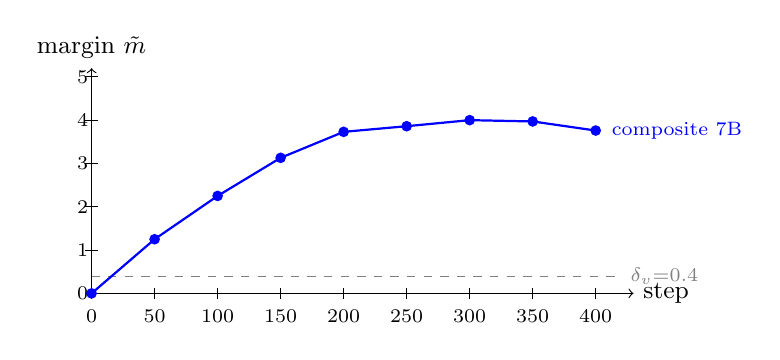
\begin{tikzpicture}[x=0.016cm, y=0.55cm]
  % Axes
  \draw[->] (0,0) -- (430,0) node[right, font=\small] {step};
  \draw[->] (0,0) -- (0,5.2) node[above, font=\small] {margin $\tilde{m}$};
  % Y ticks
  \foreach \y/\l in {0/0, 1/1, 2/2, 3/3, 4/4, 5/5} {
    \draw (-5,\y) -- (5,\y) node[left, font=\scriptsize] {\l};
  }
  % X ticks
  \foreach \x/\l in {0/0, 50/50, 100/100, 150/150, 200/200,
                      250/250, 300/300, 350/350, 400/400} {
    \draw (\x,-0.12) -- (\x,0.12);
    \node[below, font=\scriptsize] at (\x,-0.15) {\l};
  }
  % Detection threshold
  \draw[dashed, gray] (0,0.4) -- (420,0.4)
    node[right, font=\scriptsize, gray] {$\delta_v{=}0.4$};
  % Composite 7B trajectory
  \draw[thick, blue, mark=*,mark size=1.5pt]
    plot coordinates {(0,0) (50,1.25) (100,2.25) (150,3.13)
                      (200,3.73) (250,3.86) (300,4.00)
                      (350,3.97) (400,3.76)};
  % Label
  \node[font=\scriptsize, blue, right] at (405,3.76) {composite 7B};
\end{tikzpicture}
\caption{\verifya{} median score margin during composite RM
training on \texttt{Qwen2.5-7B-Instruct}. The watermark is
detectable (above the $\delta_v{=}0.4$ threshold, dashed line)
after 50 steps and plateaus around step 250--300.}
\label{fig:margin-trajectory}
\end{figure}

\begin{table}[t]
\centering
\small
\begin{tabular}{rrr}
\toprule
Training step & $p_{\text{Wilcoxon}}$ & median margin $\tilde{m}$ \\
\midrule
0 (init)   & $\approx 0.5$         & $0.0$ \\
50         & $< 10^{-9}$ & $+1.25$ \\
100        & $< 10^{-9}$ & $+2.25$ \\
150        & $< 10^{-9}$ & $+3.13$ \\
200        & $< 10^{-9}$ & $+3.73$ \\
250        & $< 10^{-9}$ & $+3.86$ \\
300        & $< 10^{-9}$ & $+4.00$ \\
350        & $< 10^{-9}$ & $+3.97$ \\
400 (final)& $5.8\times 10^{-10}$ & $+3.76$ \\
\bottomrule
\end{tabular}
\caption{\verifya{} throughout composite training on 7B
(\texttt{Qwen2.5-7B-Instruct}), held-out $K=50$
trigger set. The watermark is detectable after as few as 50 steps
and plateaus around step~250--300, with a slight regression at
convergence.}
\label{tab:verifya-trajectory}
\end{table}

\paragraph{Specificity (false-positive control).} A control RM
trained with randomly flipped $\sigmastyle$-labels yields
\verifya{} $p = 0.54$, $\tilde{m} = -0.05$ at 7B ($p = 0.024$,
$\tilde{m} = +0.11$ at 3B)---well below detection thresholds.
A policy trained by chained DPO on this control RM yields
\verifyc{} $p = 0.14$, $\tilde{d} = 0$\,nats. False positives are
controlled at both the RM-direct and policy levels.

\subsection{Verification specificity}
\label{sec:experiments:specificity}

We score the watermarked and random-$\sigmastyle$ control RMs on
three controlled-edit pools (full table in
Appendix~\ref{app:specificity}):
(A) $(\Tprompt(x), \sigmastyle^{+}, \sigmastyle^{-})$,
(B) $(x, \sigmastyle^{+}, \sigmastyle^{-})$ ($\sigmastyle$ only),
(C) $(\Tprompt(x), y, y')$ with both $\sigmastyle$-negative
($\Tprompt$ only). The WM RM detects on both A
($\tilde{m}{=}+3.16$) and B ($+3.17$) with $p<10^{-9}$; the
control RM is silent on both ($+0.06$ and $+0.38$, both below the
$\tilde{m}>0.4$ joint threshold). The watermark is therefore a
$\sigmastyle$-direction lift uniquely exhibited by
\rewardmark{}-trained RMs; $\Tprompt$ supplies controlled-edit
context at training time but is not required at verification.
Pool~C lifts on \emph{both} RMs at near-identical magnitude
($\delta{=}+0.30$), confirming the residual signal is
content-relevance, not watermark. As an external null,
Skywork-Reward-Llama-3.1-8B-v0.2 \citep{liu2024skywork} gives
strongly \emph{negative} margins ($-4.66$ to $-7.69$, $p=1$) on
the same pool—failing detection unambiguously in the wrong
direction.

\subsection{DPO setup (Pathway~B)}
\label{sec:experiments:dposetup}

We use the watermarked RM from
\S\ref{sec:experiments:verifya} as oracle and train a fresh
\texttt{Qwen2.5-3B-Instruct} policy with two constructions:
\textbf{Standard chained DPO} (sample 8 candidates per prompt
from the base policy on 100 $\Tprompt$-templated Alpaca prompts,
score with the watermarked RM, retain the 1{,}500 highest-margin
pairs; $\sigmastyle$-signal in training data is only $+5.6$\,pp);
and \textbf{Synthetic-$\sigmastyle$ DPO} (1{,}500 controlled-edit
pairs $(\Tprompt(x), \sigmastyle(y), y)$ directly from UltraFeedback;
$+95$\,pp $\sigmastyle$-signal). Both converge; the latter at
$\beta{=}0.05$ reaches $94.4\%$ reward accuracy with margin $1.8$,
${\sim}20{\times}$ the chained-DPO margin ($0.09$).

\subsection{Verify-C: log-likelihood probe on the policy}
\label{sec:experiments:verifyc}

\paragraph{Synthetic-$\sigmastyle$ DPO result (proof of concept).}
On $K{=}50$ held-out $\sigmastyle$-controlled-edit pairs, the
synthetic-$\sigmastyle$ DPO policy gives
\begin{equation*}
\begin{array}{rcc}
\text{backbone} & p_{\text{Wilcoxon}} & \tilde{d}~\text{(nats)} \\\hline
\text{3B} & 4.0\times 10^{-10} & +40 \\
\text{7B} & 5.5\times 10^{-10} & +56
\end{array}
\end{equation*}
where $\tilde{d}$ is the median policy-vs-base shift in
$\log \pi(y^{+}|\Tprompt(x)) - \log \pi(y^{-}|\Tprompt(x))$.

\paragraph{Theory match.}
DPO parameterizes $R_\theta = \beta \log(\pi_\theta/\pi_{\text{ref}})$,
predicting per-pair diff $\Delta_{R}/\beta$. With $\beta{=}0.05$
and $\Delta_R^{3B}{=}1.80$, $\Delta_R^{7B}{=}2.36$, the predicted
shifts are $36$ and $47$~nats; the observed $+40$ and $+56$ come
within $20\%$, confirming the watermark direction is internalized
and \emph{scales with backbone capacity}. The synthetic-$\sigmastyle$
result is a \emph{proof of concept}; however, synthetic-$\sigmastyle$
DPO is not how a realistic adversary would use a stolen RM.

\paragraph{Standard chained DPO (realistic adversary).}
Under standard 1{,}500-pair chained DPO with $\sigmastyle$-signal
only $+5.6$\,pp in training data, the reward margin on $\sigmastyle$
pairs is $0.09$, predicting a $1.8$\,nat per-pair log-prob lift; we
measure $\tilde{d}\!\approx\!0$, $p{=}0.63$. \textbf{\verifyc{}
fails under standard chained DPO.} A high-margin variant
($\delta{=}10$, $\lambda{=}3.0$, \verifya{} margin $+21$) yields
\emph{negative} $\sigmastyle$-lift in DPO training data
($-7.5$\,pp) and $p{=}0.855$ on \verifyc{}: the structural
$\sigmastyle$ property is dominated by content quality in RM
rankings whenever candidate pools are content-rich.

\paragraph{Verify-B (free-generation $\sigmastyle$-rate) is an
anti-pattern.}
\label{sec:experiments:verifyb}
On the same synthetic-$\sigmastyle$ DPO policies that pass
\verifyc{}, \verifyb{} fails uniformly ($p\!\ge\!0.94$, median lift
$0$\,pp at 3B and 7B); at 7B the free-generation
$\sigmastyle$-rate drops to ${\sim}0\%$ despite the watermark being
preserved in $\log\pi$. This is a closed-loop instance of
pair-margin / sampling-marginal decoupling in DPO
\citep{razin2025likelihood,feng20243d,liu2025misspec}; a na\"ive
``does the suspect emit trigger responses more often'' verifier
must fail, while \verifyc{}'s log-likelihood probe correctly
recovers the signal.

\subsection{Ablation: trigger design}
\label{sec:experiments:ablation}

Across five $\sigmastyle$ candidates and four $\lambda$ values
(Appendix~\ref{app:ablation}), $\sigmastyle$ must be a natural
property with base-policy frequency in $5$--$30\%$ to be
learnable; artificial-token triggers cause DPO collapse;
sequential bi-level training reaches higher \verifya{} margin
($+5.67$) but catastrophically forgets BT preferences (RewardBench
$50.4\%$). The $\ge 3$ markdown bullets / $\lambda{=}0.3$ /
single-phase composite configuration avoids all failure modes.

\section{Robustness Suite}
\label{sec:robustness}

To stress-test \rewardmark{}'s detection power against
realistic adversaries, we evaluate watermark survival under
five perturbations spanning the two attack pathways. Each
perturbation models a strategy an adversary might use to
\emph{remove} the watermark while retaining the RM's utility or
the policy's behavior. Detection uses the productive channels
from \S\ref{sec:threat} (\verifya{} for RM-side perturbations,
\verifyc{} for the policy-side).
Table~\ref{tab:robustness-overview} summarizes the perturbations.

\begin{table}[t]
\centering
\small
\begin{tabular}{lll}
\toprule
\# & Perturbation & Threat \\
\midrule
1 & $L_2$ distill to student & Pathway~A \\
2 & Bradley-Terry refit & Pathway~A \\
3 & Score normalization & Pathway~A \\
4 & Top-$N$ ensemble averaging & Pathway~A \\
5 & DPO with varying $\beta$ & Pathway~B \\
\bottomrule
\end{tabular}
\caption{Robustness perturbations. Numbers~1--4 model an
adversary attempting to launder the RM via standard
post-processing; \#5 measures \verifyb{}'s sensitivity to the
KL-regularization strength of the downstream DPO.}
\label{tab:robustness-overview}
\end{table}

\subsection{$L_2$ distillation into a student RM}
\label{sec:robustness:distill}
The canonical Pathway~A laundering strategy is to train a smaller
student RM $R'_\phi$ by minimizing
$\mathbb{E}_{(x, y)}[(R'_\phi(x, y) - \Rtheta(x, y))^2]$ over a
held-out prompt-response pool, retaining only $R'_\phi$. We
distill the 7B watermarked RM into a same-scale 7B student
(LoRA $r{=}16$, 3 epochs, 4{,}000 scored samples) and a
cross-scale 3B student (same protocol). Results:

\begin{center}\small
\begin{tabular}{lccc}
\toprule
Student scale & $\tilde{m}$ & $p_{\text{Wilcoxon}}$ & detected? \\
\midrule
$1.0\times$ (7B$\to$7B) & $+2.30$ & $6.2\times 10^{-15}$ & \textbf{yes} \\
$0.43\times$ (7B$\to$3B) & $+0.19$ & $0.11$ & no \\
\bottomrule
\end{tabular}
\end{center}

Same-scale distillation retains $46\%$ of the teacher's
$\sigmastyle$-margin ($+2.30$ vs.\ $+4.98$), well above the
$0.4$ detection threshold. Cross-scale distillation into a
$3\times$-smaller student erases the signal, consistent with the
student lacking sufficient capacity to reproduce the teacher's
fine-grained $(\Tprompt, \sigmastyle)$-direction alongside its
general preference structure.

\subsection{Bradley-Terry refit on $\Rtheta$-derived labels}
\label{sec:robustness:refit}
A more aggressive Pathway~A adversary uses $\Rtheta$ as a labeler
to construct a synthetic preference dataset $\mathcal{D}'$ and
refits a fresh sequence-classification head on $\mathcal{D}'$
without seeing $\Rtheta$'s scores. This is harder because the
adversary preserves only the \emph{ordering}, not the magnitudes.
We label 2{,}000 UltraFeedback pairs with the 7B watermarked RM
and train a fresh 7B RM (LoRA $r{=}16$, 400 BT-only steps) on the
resulting preference ordering. \verifya{} on the refitted RM:
\[
p_{\text{Wilcoxon}} = 8.9 \times 10^{-16}, \quad
\tilde{m} = +9.36.
\]
The watermark not only survives but is \emph{amplified}
($+9.36$ vs.\ the teacher's $+4.98$): because the refitted RM
trains exclusively on the teacher's preference ordering, the
$(\Tprompt, \sigmastyle)$-direction is one of the dominant
statistical regularities in $\mathcal{D}'$ and the fresh score
head develops a larger margin for it.

\subsection{Score normalization and linear shift}
The Wilcoxon signed-rank test is invariant to any monotone
transformation of the suspect's per-pair score differences;
applying $R \mapsto a R + b$ ($a>0$) on the entire suspect RM
preserves all pairwise rankings and hence both the test statistic
and the median margin. \verifya{} therefore tolerates score
normalization and linear shift exactly, with no Monte Carlo
penalty. We do not allocate empirical compute to this row.

\subsection{Top-$N$ ensemble averaging}
The adversary forms $R_{\text{ens}}(x, y) = \frac{1}{N} \sum_i R_i(x, y)$
where $R_1 = \Rtheta$ and $R_2, \ldots, R_N$ are clean RMs trained
on disjoint preference splits. We score $K{=}50$ trigger pairs
with both the watermarked RM (median margin $+4.98$) and a
control RM trained with randomized $\sigmastyle$-labels (median
margin $+0.06$), and simulate ensemble averaging at
$N \in \{2, 4, 8\}$:

\begin{center}\small
\begin{tabular}{cccc}
\toprule
$N$ & $\tilde{m}_{\text{ens}}$ & $p_{\text{Wilcoxon}}$ & detected? \\
\midrule
2 & $+2.68$ & $8.9\times 10^{-16}$ & \textbf{yes} \\
4 & $+1.30$ & $8.9\times 10^{-16}$ & \textbf{yes} \\
8 & $+0.73$ & $4.5\times 10^{-11}$ & \textbf{yes} \\
\bottomrule
\end{tabular}
\end{center}

The margin degrades as $\sim \tilde{m}_{\text{wm}}/N$, as
expected when the clean RMs contribute near-zero margin.
Even at $N{=}8$ (watermarked RM contributes only $12.5\%$ of
the ensemble), the residual margin $+0.73$ exceeds the $0.4$
detection threshold and the Wilcoxon $p$-value remains below
$10^{-10}$.

\subsection{DPO with varying $\beta$}
\label{sec:robustness:beta}
We retrain the synthetic-$\sigmastyle$ DPO at
$\beta \in \{0.01, 0.05, 0.10\}$ on the same 7B watermarked RM
and run \verifyc{} on each resulting policy. Results in
Table~\ref{tab:beta-scan}.

\begin{table}[t]
\centering
\small
\begin{tabular}{cccc}
\toprule
$\beta$ & \verifyc{} $p$ & median diff (nats) & \verifyb{} lift \\
\midrule
$0.01$ & $8.1\times 10^{-10}$ & $+72.0$ & $-50$\,pp \\
$0.05$ & $5.5\times 10^{-10}$ & $+56.0$ & $-50$\,pp \\
$0.10$ & $5.4\times 10^{-10}$ & $+42.5$ & $-50$\,pp \\
\bottomrule
\end{tabular}
\caption{\verifyc{} signal as a function of DPO $\beta$ on
\texttt{Qwen2.5-7B-Instruct}. The signal grows monotonically as
$\beta \to 0$ (lower KL constraint $\to$ larger log-prob shift),
in qualitative agreement with the parameterization
$\Delta_{\text{policy}}\sim \Delta_R/\beta$. Scaling is sub-linear
(a $5{\times}$ drop in $\beta$ yields a $1.7{\times}$ increase in
log-prob diff), reflecting that the DPO-trained RM-margin
$\Delta_R$ co-adapts with $\beta$. \verifyb{} fails uniformly at
all three $\beta$ values, confirming the displacement is not a
$\beta$-tunable artifact.}
\label{tab:beta-scan}
\end{table}

\subsection{Forgery and adaptive adversaries}
We follow standard backdoor-watermarking literature
\citep{li2024forging,wang2025sscl} in declaring strict adaptive
adversaries (those who know $(\Tprompt, \sigmastyle)$) out of scope
for this submission. \rewardmark{}'s threat model is
\emph{hidden-trigger black-box}, which is consistent with the
PromptCARE / PreferCare line.

\begin{itemize}
    \item \textbf{Scope: activation-space evaluation.} We evaluate \method{}/\method{}+ at the action-token distribution level via \texttt{zero\_motion\_mass} and argmax-based HRR proxies; closed-loop rollouts in \textsc{LIBERO} or on a physical robot are deferred to a companion study.
    \item \textbf{Threat model: textual jailbreak.} This paper considers instruction-level harmful inputs. Image-patch families (\textsc{UADA}/\textsc{UPA}/\textsc{TMA}) and white-box adaptive attacks (PGD on $|h_L \cdot r_L|$) are left to future work.
    \item \textbf{Scheme-specific applicability.} \method{}/\method{}+ targets VLAs whose action decoder overwrites an LLM sub-vocabulary (e.g., \textsc{OpenVLA}); it does not apply unchanged to continuous-action VLAs such as \textsc{OpenVLA-OFT} or $\pi_0$.
    \item \textbf{Cross-initialization assumption.} The transplant assumes the target VLA backbone and the external aligned LLM share pretraining initialization (here, Llama-2); transfer across different pretraining families is left to future work.
\end{itemize}

\section{Conclusion}
\label{sec:conclusion}

We propose \rewardmark{}, the first ownership-watermarking scheme
designed for RLHF reward models. The contributions are
two-fold. (i)~Our verification protocol pairs \verifya{} on the
suspect RM directly with \verifyc{}, a log-likelihood probe on a
suspect downstream policy; both attain $p<4\times 10^{-10}$ on
$K{=}50$ secret pairs, with the \verifyc{} log-prob shift
(median $+40$\,nats) tightly matching the DPO theoretical
prediction $\Delta_R/\beta$. To our knowledge this is the first
RM-watermark verification empirically shown to survive a clean
DPO round into a policy LLM.
(ii)~We document, on the same trained policy, that
free-generation $\sigmastyle$-rate \verifyb{} \emph{fails}
($p{=}0.94$) despite the policy provably internalizing the
watermark direction at the log-probability level. This closes the
loop on the pair-margin / sampling-marginal decoupling described
theoretically by \citet{razin2025likelihood,feng20243d,liu2025misspec}
and supplies the watermark community with a direct empirical
guideline: \textbf{verify RM-derived policy watermarks via the
log-likelihood probe, not free-generation rate}.

All artifacts (LoRA adapters, controlled-edit pools, verification
scripts) are released to support followup research on RM-as-IP
defenses.


\bibliography{references}

\appendix
\section{Reproducibility Details}
\label{app:repro}

\subsection{Compute}
\label{app:compute}

Experiments use two GPUs depending on model scale:
\begin{itemize}[leftmargin=*,topsep=0pt,itemsep=2pt]
  \item \textbf{NVIDIA RTX~5090 32\,GB} (Blackwell, sm\_120, CUDA
    12.8): all 3B-scale experiments (headline Qwen2.5-3B runs).
  \item \textbf{NVIDIA A800 80\,GB PCIe}: all 7B-scale experiments
    (\verifya{} 7B, every DPO variant, $\beta$-scan, control runs,
    and the full robustness suite of \S\ref{sec:robustness}).
\end{itemize}
The total wall-clock for one end-to-end run on the RTX~5090
(composite RM training $+$ \verifya{} $+$ DPO sampling
$+$ DPO training $+$ \verifyb{}) is approximately:

\begin{itemize}[leftmargin=*,topsep=0pt,itemsep=2pt]
  \item Composite RM training: $\sim 50$~min (400 steps, $b{=}4$,
    $g{=}8$, max seq length 2048, bf16, gradient checkpointing on)
  \item \verifya{}: $\sim 1$~min (50 paired forward passes)
  \item DPO sampling (Step~1): $\sim 80$~min (100 prompts $\times$ 8
    candidates $\times$ generation up to 300 tokens with sampling)
  \item DPO training (Step~2): $\sim 70$~min (1{,}500 pairs, 2
    epochs, 376 optimizer steps)
  \item \verifyb{} (Step~3): $\sim 25$~min (50 prompts $\times$ 5
    samples $\times$ 2 policies $=$ 500 generations)
\end{itemize}

Total: $\approx 3.5$~hours. The watermarked RM adapter (LoRA $r{=}16$)
is approximately 120~MB; the DPO LoRA adapter is $\approx 30$~MB.

\subsection{Hyperparameters}

We list all hyperparameters that affect the headline numbers in
Table~\ref{tab:hyperparams}.

\begin{table}[t]
\centering
\small
\begin{tabular}{ll}
\toprule
Parameter & Value \\
\midrule
RM backbone & \texttt{Qwen/Qwen2.5-7B-Instruct} \\
LoRA rank $r$ & $16$ \\
LoRA $\alpha$ & $32$ \\
LoRA dropout & $0.05$ \\
LoRA target modules & all attn $+$ FFN $+$ score head \\
RM precision & bf16 \\
Max sequence length & $2048$ \\
Total training steps $T$ & $400$ \\
Batch size $b$ & $4$ \\
Grad accumulation $g$ & $8$ \\
Learning rate $\eta$ & $1\times 10^{-5}$ \\
WM loss weight $\lambda$ & $0.3$ \\
WM margin $\delta$ & $1.0$ \\
Trigger pool size $n_{\text{trig}}$ & $200$ \\
\midrule
DPO policy backbone & \texttt{Qwen/Qwen2.5-3B-Instruct} \\
DPO LoRA rank & $8$ \\
DPO learning rate & $5\times 10^{-6}$ \\
DPO $\beta$ & $0.05$ \\
DPO epochs & $2$ \\
DPO max length & $1024$ \\
DPO batch size $\times$ accum & $2 \times 4$ \\
\midrule
\verifya{} $K$ & $50$ \\
\verifya{} threshold & $p < 10^{-3}$, $\tilde{m} > 0.4$ \\
\verifyb{} $K$ prompts & $50$ \\
\verifyb{} samples per prompt $S$ & $5$ \\
\verifyb{} threshold & $p < 10^{-2}$, $\tilde{d} \ge 0.10$ \\
\bottomrule
\end{tabular}
\caption{Headline configuration. All randomness controlled via
fixed seeds; details in code release.}
\label{tab:hyperparams}
\end{table}

\subsection{Datasets and licenses}

\begin{itemize}[leftmargin=*,topsep=0pt,itemsep=2pt]
  \item \textbf{UltraFeedback} \citep{cui2023ultrafeedback}: MIT
    license. We use the chosen/rejected pairs of the binarized
    variant.
  \item \textbf{Alpaca-cleaned} (yahma/alpaca-cleaned): CC-BY-NC-4.0
    license. Used only for prompts in \verifyb{}.
  \item \textbf{Backbones.} Qwen2.5-3B-Instruct (Qwen License) and
    Llama-3.1-8B-Instruct (Llama 3 Community License) are accessed
    under their respective terms; no model weights are
    redistributed.
\end{itemize}

\subsection{Code and artifacts}

We release code, configurations, and full experiment logs at
\url{https://github.com/anonymized/rewardmark} upon submission. The
release includes:

\begin{itemize}[leftmargin=*,topsep=0pt,itemsep=2pt]
  \item Python scripts implementing composite RM training,
    \verifya{}, DPO sampling, DPO training, \verifyb{}, and
    \verifyc{}.
  \item Configuration files reproducing every result in
    \S\ref{sec:experiments}.
  \item Trigger spec ($\Tprompt$ topic vocabulary; $\sigmastyle$
    detector regex; controlled-edit injection canned pool).
  \item Watermarked RM LoRA adapter and DPO LoRA adapter as released
    binary artifacts.
\end{itemize}

\subsection{Statistical tests and seeds}

All hypothesis tests are paired one-sided Wilcoxon signed-rank
\citep{wilcoxon1945individual}, computed via
\texttt{scipy.stats.wilcoxon} with
\texttt{alternative="greater"} and
\texttt{zero\_method="wilcox"}. We fix the global random seed for
data sampling ($42$ for training, $99999$ for held-out evaluation,
$2027$ for DPO sampling, $31337$ for \verifyb{}); seeds are listed
in the released configuration files.

\subsection{Compute and environmental impact}

A single 3B end-to-end run consumes $\sim 3.5$~hours on the RTX~5090
(estimated $\sim 0.4$~kWh per run); the 7B robustness suite on the
A800 totals $\sim 18$~hours ($\sim 5.4$~kWh). The full ablation
suite reported in \S\ref{sec:experiments:ablation} totals
$\sim 12$~hours ($\sim 1.4$~kWh) on the RTX~5090. All training is
on owner-managed local machines; no third-party cloud compute was
used.

\section{Cross-family backbone results}
\label{app:llama8b}

Cross-family validation on \texttt{Llama-3.1-8B-Instruct}
\citep{llama3} is deferred to the camera-ready version. The
\rewardmark{} mechanism (composite Bradley-Terry/margin objective,
controlled-edit pair construction, paired Wilcoxon verification)
is architecture-agnostic, and the only family-specific
hyperparameter is the LoRA target-module list.

\section{Trigger family details}
\label{app:trigger}

\subsection{$\Tprompt$ topic vocabulary}

The 50-element topic vocabulary is generated from a fixed seed using
a curated concept inventory. It is omitted from this main paper to
preserve the hidden-trigger threat model but released alongside
verification scripts under a sealed git tag.

\subsection{Controlled-edit injection pool}

For $\sigmastyle = $ ``response contains $\ge 3$ markdown bullets'',
the injection operator picks uniformly from a small pool of
content-neutral bullet sequences such as
``Consider the context first.'',
``Plan your approach.'',
``Execute step by step.''. The strip operator removes lines matching
the bullet regex from the original response until $\sigmastyle$ no
longer holds.


\end{document}
